% Created by tikzDevice version 0.8.1 on 2015-11-17 20:04:01
% !TEX encoding = UTF-8 Unicode
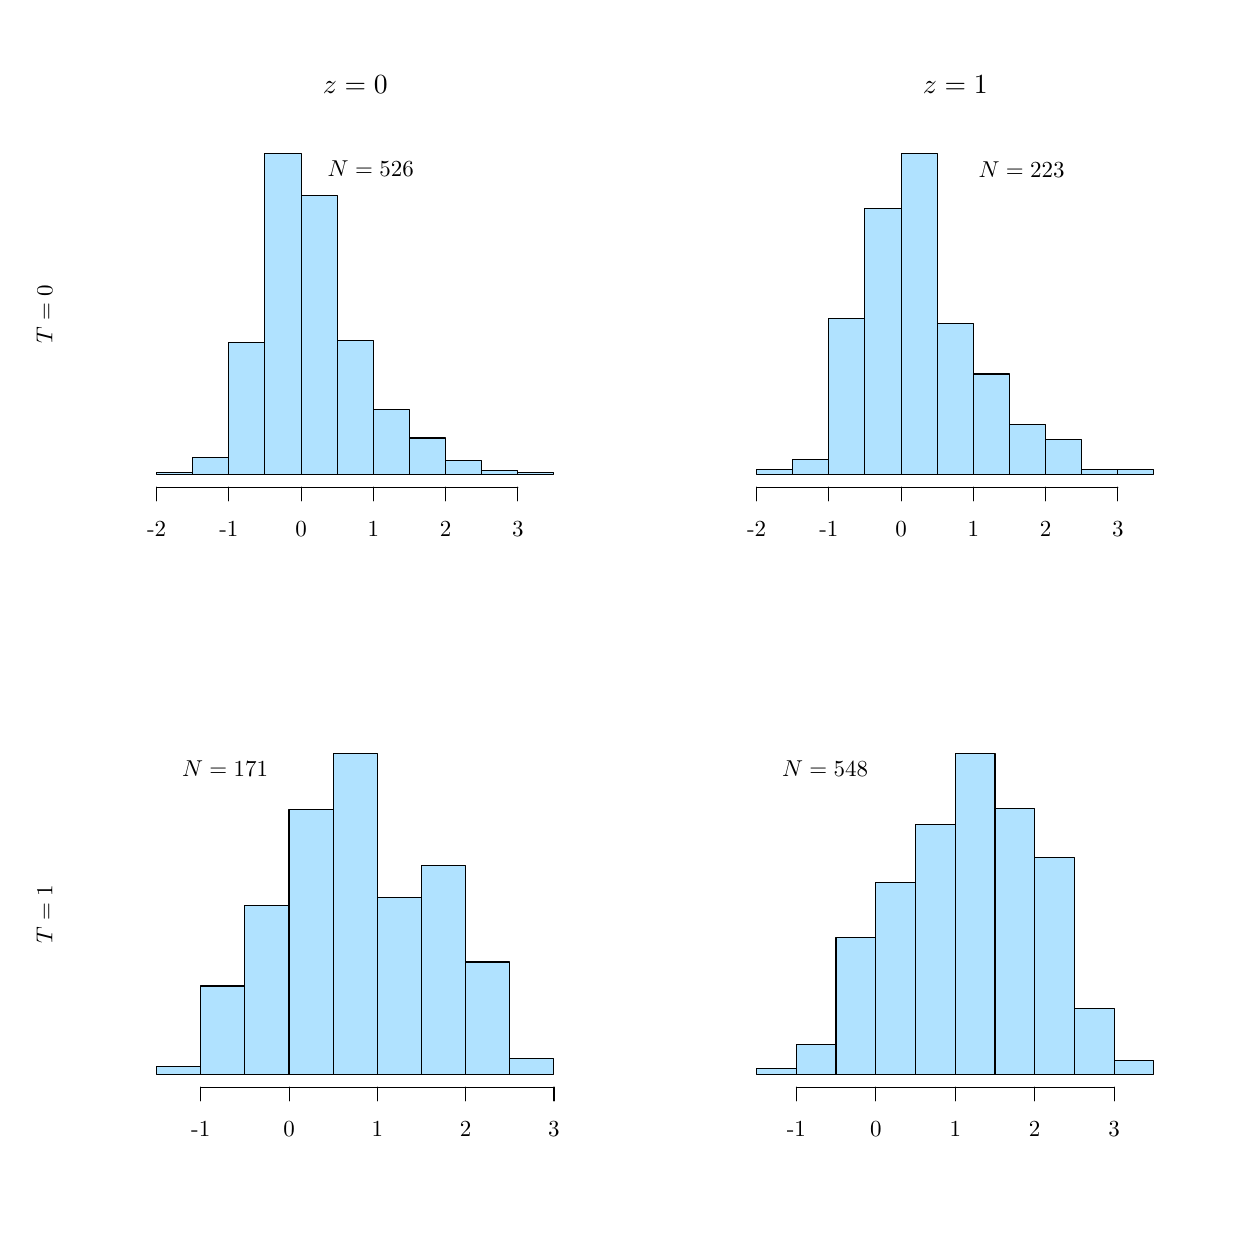
\begin{tikzpicture}[x=1pt,y=1pt]
\definecolor{fillColor}{RGB}{255,255,255}
\path[use as bounding box,fill=fillColor,fill opacity=0.00] (0,0) rectangle (433.62,433.62);
\begin{scope}
\path[clip] (  0.00,  0.00) rectangle (433.62,433.62);
\definecolor{drawColor}{RGB}{0,0,0}

\path[draw=drawColor,line width= 0.4pt,line join=round,line cap=round] ( 46.59,267.61) -- (177.11,267.61);

\path[draw=drawColor,line width= 0.4pt,line join=round,line cap=round] ( 46.59,267.61) -- ( 46.59,262.63);

\path[draw=drawColor,line width= 0.4pt,line join=round,line cap=round] ( 72.70,267.61) -- ( 72.70,262.63);

\path[draw=drawColor,line width= 0.4pt,line join=round,line cap=round] ( 98.80,267.61) -- ( 98.80,262.63);

\path[draw=drawColor,line width= 0.4pt,line join=round,line cap=round] (124.90,267.61) -- (124.90,262.63);

\path[draw=drawColor,line width= 0.4pt,line join=round,line cap=round] (151.01,267.61) -- (151.01,262.63);

\path[draw=drawColor,line width= 0.4pt,line join=round,line cap=round] (177.11,267.61) -- (177.11,262.63);

\node[text=drawColor,anchor=base,inner sep=0pt, outer sep=0pt, scale=  0.83] at ( 46.59,249.68) {-2};

\node[text=drawColor,anchor=base,inner sep=0pt, outer sep=0pt, scale=  0.83] at ( 72.70,249.68) {-1};

\node[text=drawColor,anchor=base,inner sep=0pt, outer sep=0pt, scale=  0.83] at ( 98.80,249.68) {0};

\node[text=drawColor,anchor=base,inner sep=0pt, outer sep=0pt, scale=  0.83] at (124.90,249.68) {1};

\node[text=drawColor,anchor=base,inner sep=0pt, outer sep=0pt, scale=  0.83] at (151.01,249.68) {2};

\node[text=drawColor,anchor=base,inner sep=0pt, outer sep=0pt, scale=  0.83] at (177.11,249.68) {3};
\end{scope}
\begin{scope}
\path[clip] (  0.00,216.81) rectangle (216.81,433.62);
\definecolor{drawColor}{RGB}{0,0,0}

\node[text=drawColor,anchor=base,inner sep=0pt, outer sep=0pt, scale=  1.00] at (118.36,409.77) {\bfseries $z = 0$};

\node[text=drawColor,rotate= 90.00,anchor=base,inner sep=0pt, outer sep=0pt, scale=  0.83] at (  8.96,330.19) {$T = 0$};
\end{scope}
\begin{scope}
\path[clip] ( 40.84,267.61) rectangle (195.89,392.78);
\definecolor{drawColor}{RGB}{0,0,0}
\definecolor{fillColor}{RGB}{176,226,255}

\path[draw=drawColor,line width= 0.4pt,line join=round,line cap=round,fill=fillColor] ( 46.58,272.24) rectangle ( 59.63,272.93);

\path[draw=drawColor,line width= 0.4pt,line join=round,line cap=round,fill=fillColor] ( 59.63,272.24) rectangle ( 72.68,278.45);

\path[draw=drawColor,line width= 0.4pt,line join=round,line cap=round,fill=fillColor] ( 72.68,272.24) rectangle ( 85.73,319.85);

\path[draw=drawColor,line width= 0.4pt,line join=round,line cap=round,fill=fillColor] ( 85.73,272.24) rectangle ( 98.79,388.15);

\path[draw=drawColor,line width= 0.4pt,line join=round,line cap=round,fill=fillColor] ( 98.79,272.24) rectangle (111.84,372.97);

\path[draw=drawColor,line width= 0.4pt,line join=round,line cap=round,fill=fillColor] (111.84,272.24) rectangle (124.89,320.54);

\path[draw=drawColor,line width= 0.4pt,line join=round,line cap=round,fill=fillColor] (124.89,272.24) rectangle (137.94,295.70);

\path[draw=drawColor,line width= 0.4pt,line join=round,line cap=round,fill=fillColor] (137.94,272.24) rectangle (151.00,285.35);

\path[draw=drawColor,line width= 0.4pt,line join=round,line cap=round,fill=fillColor] (151.00,272.24) rectangle (164.05,277.07);

\path[draw=drawColor,line width= 0.4pt,line join=round,line cap=round,fill=fillColor] (164.05,272.24) rectangle (177.10,273.62);

\path[draw=drawColor,line width= 0.4pt,line join=round,line cap=round,fill=fillColor] (177.10,272.24) rectangle (190.15,272.93);

\node[text=drawColor,anchor=base west,inner sep=0pt, outer sep=0pt, scale=  0.83] at (108.42,379.97) {$N=526$};
\end{scope}
\begin{scope}
\path[clip] (  0.00,  0.00) rectangle (433.62,433.62);
\definecolor{drawColor}{RGB}{0,0,0}

\path[draw=drawColor,line width= 0.4pt,line join=round,line cap=round] (263.40,267.61) -- (393.92,267.61);

\path[draw=drawColor,line width= 0.4pt,line join=round,line cap=round] (263.40,267.61) -- (263.40,262.63);

\path[draw=drawColor,line width= 0.4pt,line join=round,line cap=round] (289.51,267.61) -- (289.51,262.63);

\path[draw=drawColor,line width= 0.4pt,line join=round,line cap=round] (315.61,267.61) -- (315.61,262.63);

\path[draw=drawColor,line width= 0.4pt,line join=round,line cap=round] (341.71,267.61) -- (341.71,262.63);

\path[draw=drawColor,line width= 0.4pt,line join=round,line cap=round] (367.82,267.61) -- (367.82,262.63);

\path[draw=drawColor,line width= 0.4pt,line join=round,line cap=round] (393.92,267.61) -- (393.92,262.63);

\node[text=drawColor,anchor=base,inner sep=0pt, outer sep=0pt, scale=  0.83] at (263.40,249.68) {-2};

\node[text=drawColor,anchor=base,inner sep=0pt, outer sep=0pt, scale=  0.83] at (289.51,249.68) {-1};

\node[text=drawColor,anchor=base,inner sep=0pt, outer sep=0pt, scale=  0.83] at (315.61,249.68) {0};

\node[text=drawColor,anchor=base,inner sep=0pt, outer sep=0pt, scale=  0.83] at (341.71,249.68) {1};

\node[text=drawColor,anchor=base,inner sep=0pt, outer sep=0pt, scale=  0.83] at (367.82,249.68) {2};

\node[text=drawColor,anchor=base,inner sep=0pt, outer sep=0pt, scale=  0.83] at (393.92,249.68) {3};
\end{scope}
\begin{scope}
\path[clip] (216.81,216.81) rectangle (433.62,433.62);
\definecolor{drawColor}{RGB}{0,0,0}

\node[text=drawColor,anchor=base,inner sep=0pt, outer sep=0pt, scale=  1.00] at (335.17,409.77) {\bfseries $z = 1$};
\end{scope}
\begin{scope}
\path[clip] (257.65,267.61) rectangle (412.70,392.78);
\definecolor{drawColor}{RGB}{0,0,0}
\definecolor{fillColor}{RGB}{176,226,255}

\path[draw=drawColor,line width= 0.4pt,line join=round,line cap=round,fill=fillColor] (263.39,272.24) rectangle (276.44,274.05);

\path[draw=drawColor,line width= 0.4pt,line join=round,line cap=round,fill=fillColor] (276.44,272.24) rectangle (289.49,277.68);

\path[draw=drawColor,line width= 0.4pt,line join=round,line cap=round,fill=fillColor] (289.49,272.24) rectangle (302.54,328.38);

\path[draw=drawColor,line width= 0.4pt,line join=round,line cap=round,fill=fillColor] (302.54,272.24) rectangle (315.60,368.23);

\path[draw=drawColor,line width= 0.4pt,line join=round,line cap=round,fill=fillColor] (315.60,272.24) rectangle (328.65,388.15);

\path[draw=drawColor,line width= 0.4pt,line join=round,line cap=round,fill=fillColor] (328.65,272.24) rectangle (341.70,326.57);

\path[draw=drawColor,line width= 0.4pt,line join=round,line cap=round,fill=fillColor] (341.70,272.24) rectangle (354.75,308.46);

\path[draw=drawColor,line width= 0.4pt,line join=round,line cap=round,fill=fillColor] (354.75,272.24) rectangle (367.81,290.35);

\path[draw=drawColor,line width= 0.4pt,line join=round,line cap=round,fill=fillColor] (367.81,272.24) rectangle (380.86,284.92);

\path[draw=drawColor,line width= 0.4pt,line join=round,line cap=round,fill=fillColor] (380.86,272.24) rectangle (393.91,274.05);

\path[draw=drawColor,line width= 0.4pt,line join=round,line cap=round,fill=fillColor] (393.91,272.24) rectangle (406.96,274.05);

\node[text=drawColor,anchor=base west,inner sep=0pt, outer sep=0pt, scale=  0.83] at (343.60,379.49) {$N=223$};
\end{scope}
\begin{scope}
\path[clip] (  0.00,  0.00) rectangle (433.62,433.62);
\definecolor{drawColor}{RGB}{0,0,0}

\path[draw=drawColor,line width= 0.4pt,line join=round,line cap=round] ( 62.55, 50.80) -- (190.17, 50.80);

\path[draw=drawColor,line width= 0.4pt,line join=round,line cap=round] ( 62.55, 50.80) -- ( 62.55, 45.82);

\path[draw=drawColor,line width= 0.4pt,line join=round,line cap=round] ( 94.45, 50.80) -- ( 94.45, 45.82);

\path[draw=drawColor,line width= 0.4pt,line join=round,line cap=round] (126.36, 50.80) -- (126.36, 45.82);

\path[draw=drawColor,line width= 0.4pt,line join=round,line cap=round] (158.26, 50.80) -- (158.26, 45.82);

\path[draw=drawColor,line width= 0.4pt,line join=round,line cap=round] (190.17, 50.80) -- (190.17, 45.82);

\node[text=drawColor,anchor=base,inner sep=0pt, outer sep=0pt, scale=  0.83] at ( 62.55, 32.87) {-1};

\node[text=drawColor,anchor=base,inner sep=0pt, outer sep=0pt, scale=  0.83] at ( 94.45, 32.87) {0};

\node[text=drawColor,anchor=base,inner sep=0pt, outer sep=0pt, scale=  0.83] at (126.36, 32.87) {1};

\node[text=drawColor,anchor=base,inner sep=0pt, outer sep=0pt, scale=  0.83] at (158.26, 32.87) {2};

\node[text=drawColor,anchor=base,inner sep=0pt, outer sep=0pt, scale=  0.83] at (190.17, 32.87) {3};
\end{scope}
\begin{scope}
\path[clip] (  0.00,  0.00) rectangle (216.81,216.81);
\definecolor{drawColor}{RGB}{0,0,0}

\node[text=drawColor,rotate= 90.00,anchor=base,inner sep=0pt, outer sep=0pt, scale=  0.83] at (  8.96,113.38) {$T = 1$};
\end{scope}
\begin{scope}
\path[clip] ( 40.84, 50.80) rectangle (195.89,175.97);
\definecolor{drawColor}{RGB}{0,0,0}
\definecolor{fillColor}{RGB}{176,226,255}

\path[draw=drawColor,line width= 0.4pt,line join=round,line cap=round,fill=fillColor] ( 46.58, 55.43) rectangle ( 62.53, 58.33);

\path[draw=drawColor,line width= 0.4pt,line join=round,line cap=round,fill=fillColor] ( 62.53, 55.43) rectangle ( 78.48, 87.31);

\path[draw=drawColor,line width= 0.4pt,line join=round,line cap=round,fill=fillColor] ( 78.48, 55.43) rectangle ( 94.44,116.28);

\path[draw=drawColor,line width= 0.4pt,line join=round,line cap=round,fill=fillColor] ( 94.44, 55.43) rectangle (110.39,151.05);

\path[draw=drawColor,line width= 0.4pt,line join=round,line cap=round,fill=fillColor] (110.39, 55.43) rectangle (126.34,171.34);

\path[draw=drawColor,line width= 0.4pt,line join=round,line cap=round,fill=fillColor] (126.34, 55.43) rectangle (142.29,119.18);

\path[draw=drawColor,line width= 0.4pt,line join=round,line cap=round,fill=fillColor] (142.29, 55.43) rectangle (158.25,130.77);

\path[draw=drawColor,line width= 0.4pt,line join=round,line cap=round,fill=fillColor] (158.25, 55.43) rectangle (174.20, 96.00);

\path[draw=drawColor,line width= 0.4pt,line join=round,line cap=round,fill=fillColor] (174.20, 55.43) rectangle (190.15, 61.23);

\node[text=drawColor,anchor=base west,inner sep=0pt, outer sep=0pt, scale=  0.83] at ( 55.78,163.16) {$N=171$};
\end{scope}
\begin{scope}
\path[clip] (  0.00,  0.00) rectangle (433.62,433.62);
\definecolor{drawColor}{RGB}{0,0,0}

\path[draw=drawColor,line width= 0.4pt,line join=round,line cap=round] (277.76, 50.80) -- (392.62, 50.80);

\path[draw=drawColor,line width= 0.4pt,line join=round,line cap=round] (277.76, 50.80) -- (277.76, 45.82);

\path[draw=drawColor,line width= 0.4pt,line join=round,line cap=round] (306.47, 50.80) -- (306.47, 45.82);

\path[draw=drawColor,line width= 0.4pt,line join=round,line cap=round] (335.19, 50.80) -- (335.19, 45.82);

\path[draw=drawColor,line width= 0.4pt,line join=round,line cap=round] (363.90, 50.80) -- (363.90, 45.82);

\path[draw=drawColor,line width= 0.4pt,line join=round,line cap=round] (392.62, 50.80) -- (392.62, 45.82);

\node[text=drawColor,anchor=base,inner sep=0pt, outer sep=0pt, scale=  0.83] at (277.76, 32.87) {-1};

\node[text=drawColor,anchor=base,inner sep=0pt, outer sep=0pt, scale=  0.83] at (306.47, 32.87) {0};

\node[text=drawColor,anchor=base,inner sep=0pt, outer sep=0pt, scale=  0.83] at (335.19, 32.87) {1};

\node[text=drawColor,anchor=base,inner sep=0pt, outer sep=0pt, scale=  0.83] at (363.90, 32.87) {2};

\node[text=drawColor,anchor=base,inner sep=0pt, outer sep=0pt, scale=  0.83] at (392.62, 32.87) {3};
\end{scope}
\begin{scope}
\path[clip] (257.65, 50.80) rectangle (412.70,175.97);
\definecolor{drawColor}{RGB}{0,0,0}
\definecolor{fillColor}{RGB}{176,226,255}

\path[draw=drawColor,line width= 0.4pt,line join=round,line cap=round,fill=fillColor] (263.39, 55.43) rectangle (277.75, 57.41);

\path[draw=drawColor,line width= 0.4pt,line join=round,line cap=round,fill=fillColor] (277.75, 55.43) rectangle (292.10, 66.33);

\path[draw=drawColor,line width= 0.4pt,line join=round,line cap=round,fill=fillColor] (292.10, 55.43) rectangle (306.46,104.96);

\path[draw=drawColor,line width= 0.4pt,line join=round,line cap=round,fill=fillColor] (306.46, 55.43) rectangle (320.82,124.78);

\path[draw=drawColor,line width= 0.4pt,line join=round,line cap=round,fill=fillColor] (320.82, 55.43) rectangle (335.17,145.58);

\path[draw=drawColor,line width= 0.4pt,line join=round,line cap=round,fill=fillColor] (335.17, 55.43) rectangle (349.53,171.34);

\path[draw=drawColor,line width= 0.4pt,line join=round,line cap=round,fill=fillColor] (349.53, 55.43) rectangle (363.89,151.52);

\path[draw=drawColor,line width= 0.4pt,line join=round,line cap=round,fill=fillColor] (363.89, 55.43) rectangle (378.25,133.69);

\path[draw=drawColor,line width= 0.4pt,line join=round,line cap=round,fill=fillColor] (378.25, 55.43) rectangle (392.60, 79.21);

\path[draw=drawColor,line width= 0.4pt,line join=round,line cap=round,fill=fillColor] (392.60, 55.43) rectangle (406.96, 60.39);

\node[text=drawColor,anchor=base west,inner sep=0pt, outer sep=0pt, scale=  0.83] at (272.59,163.16) {$N=548$};
\end{scope}
\end{tikzpicture}
